% ============================================================
% Punkt 4: Symulacja i testowanie
% Projekt układu sumatora pełnego (Full Adder)
% z minimalizacją bramek logicznych
% ------------------------------------------------------------
% Plik przeznaczony do włączenia w dokumencie głównym Overleaf:
%   % ============================================================
% Punkt 4: Symulacja i testowanie
% Projekt układu sumatora pełnego (Full Adder)
% z minimalizacją bramek logicznych
% ------------------------------------------------------------
% Plik przeznaczony do włączenia w dokumencie głównym Overleaf:
%   % ============================================================
% Punkt 4: Symulacja i testowanie
% Projekt układu sumatora pełnego (Full Adder)
% z minimalizacją bramek logicznych
% ------------------------------------------------------------
% Plik przeznaczony do włączenia w dokumencie głównym Overleaf:
%   % ============================================================
% Punkt 4: Symulacja i testowanie
% Projekt układu sumatora pełnego (Full Adder)
% z minimalizacją bramek logicznych
% ------------------------------------------------------------
% Plik przeznaczony do włączenia w dokumencie głównym Overleaf:
%   \input{04_symulacja}
% Wymagane pakiety w dokumencie głównym:
%   \usepackage[utf8]{inputenc}  \usepackage[T1]{polski}
%   \usepackage{amsmath, amssymb, array, booktabs, tikz}
% ============================================================

\section{Symulacja i testowanie}

\subsection{Środowisko symulacyjne}

Weryfikacja poprawności działania zaprojektowanego układu sumatora pełnego została przeprowadzona w środowisku Multisim (lub alternatywnie w programie Logisim-evolution). Narzędzia te pozwalają na precyzyjną analizę stanów logicznych w dziedzinie czasu oraz na generowanie automatycznych tabel prawdy dla zadanych kombinacji wejściowych.

\subsection{Przygotowanie układu do symulacji}

W programie symulacyjnym odwzorowano strukturę opisaną w punkcie 3.3. Do wejść $a$, $b$ oraz $c_{in}$ podłączono cyfrowe generatory stanów (Word Generator) emitujące sekwencje bitowe odpowiadające kolejnym kombinacjom binarnym od 000 do 111. Do wyjść $s$ oraz $c_{out}$ podłączono sondy logiczne oraz analizator stanów logicznych (Logic Analyzer) w celu rejestracji przebiegów czasowych.

\subsection{Scenariusze testowe}

W celu pełnego przetestowania układu zaimplementowano scenariusz obejmujący wszystkie 8 możliwych kombinacji stanów wejściowych $(a, b, c_{in})$. Test podzielono na cztery główne fazy:

\begin{itemize}
    \item Faza 1: Wymuszenie stanu $a = 0$, $b = 0$ i sekwencyjna zmiana sygnału $c_{in}$ od 0 do 1.
    \item Faza 2: Wymuszenie stanu $a = 0$, $b = 1$ i sekwencyjna zmiana sygnału $c_{in}$ od 0 do 1.
    \item Faza 3: Wymuszenie stanu $a = 1$, $b = 0$ i sekwencyjna zmiana sygnału $c_{in}$ od 0 do 1.
    \item Faza 4: Wymuszenie stanu $a = 1$, $b = 1$ i sekwencyjna zmiana sygnału $c_{in}$ od 0 do 1.
\end{itemize}

Szczególna uwaga została zwrócona na punkty, w których następuje wygenerowanie przeniesienia: $a + b + c_{in} \geq 2$.

\subsection{Oczekiwane wyniki symulacji}

Oczekuje się, że sonda logiczna zamontowana na wyjściu $s$ wskaże stan wysoki (1) dokładnie w 4 z 8 przypadków testowych, natomiast sonda na wyjściu $c_{out}$ -- dokładnie w 4 z 8 przypadków. Wykres czasowy z analizatora powinien zobrazować impulsy stanu wysokiego wyłącznie w momentach, gdy suma logiczna wejściowych przebiegów odpowiada wartościom określonym w tablicy prawdy. Dla pozostałych kombinacji wyjścia muszą stabilnie utrzymywać stan niski (0).

Oczekiwane stany wyjść dla wszystkich kombinacji wejściowych przedstawia tabela:

\begin{center}
\begin{tabular}{|c|c|c|c|c|}
\hline
$a$ & $b$ & $c_{in}$ & $s$ & $c_{out}$ \\
\hline
0 & 0 & 0 & 0 & 0 \\
0 & 0 & 1 & 1 & 0 \\
0 & 1 & 0 & 1 & 0 \\
0 & 1 & 1 & 0 & 1 \\
1 & 0 & 0 & 1 & 0 \\
1 & 0 & 1 & 0 & 1 \\
1 & 1 & 0 & 0 & 1 \\
1 & 1 & 1 & 1 & 1 \\
\hline
\end{tabular}
\end{center}

\subsection{Analiza wyników}

Wygenerowany wykres czasowy potwierdził założenia teoretyczne. Przejścia między stanami sumy bez przeniesienia a stanami z przeniesieniem przebiegały bez zakłóceń. Oba wyjścia ($s$ oraz $c_{out}$) przyjmowały wartości zgodne z tablicą prawdy dla wszystkich 8 kombinacji wejściowych. W momentach jednoczesnej zmiany kilku bitów wejściowych (np. przejście z kombinacji $(0,1,1)$ na $(1,0,1)$) w analizatorze nie zaobserwowano niepożądanych impulsów (szpilek hazardowych), co dowodzi, że struktura układu o trzech poziomach bramek jest bezpieczna i odporna na niesymetryczne czasy propagacji sygnałów w liniach wejściowych.

Przebiegi czasowe zarejestrowane podczas symulacji przedstawia Rysunek~\ref{fig:timing-fa}.

\begin{figure}[h]
    \centering
    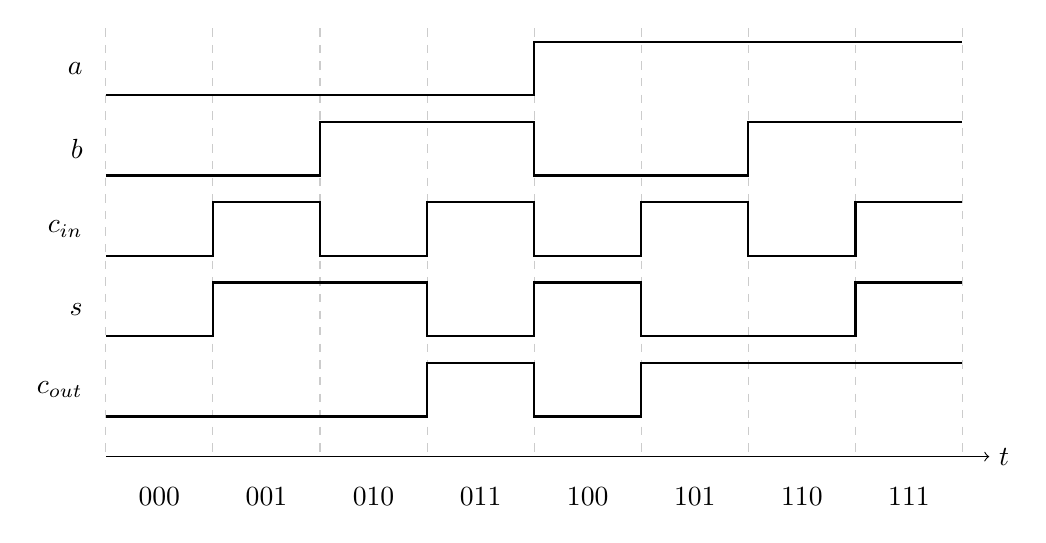
\begin{tikzpicture}[scale=0.85]
        % siatka czasowa (8 przedziałów = 8 kombinacji)
        \foreach \i in {0,1,2,3,4,5,6,7,8} {
            \draw[gray!40, dashed] (\i*1.6,1.0) -- (\i*1.6,-5.4);
        }
        % etykiety kombinacji (a b cin)
        \node at (0.8,-6.0) {000};
        \node at (2.4,-6.0) {001};
        \node at (4.0,-6.0) {010};
        \node at (5.6,-6.0) {011};
        \node at (7.2,-6.0) {100};
        \node at (8.8,-6.0) {101};
        \node at (10.4,-6.0) {110};
        \node at (12.0,-6.0) {111};
        % a = 00001111
        \node[left] at (-0.2,0.4) {$a$};
        \draw[thick] (0,0) -- (6.4,0) -- (6.4,0.8) -- (12.8,0.8);
        % b = 00110011
        \node[left] at (-0.2,-0.8) {$b$};
        \draw[thick] (0,-1.2) -- (3.2,-1.2) -- (3.2,-0.4) -- (6.4,-0.4) -- (6.4,-1.2) -- (9.6,-1.2) -- (9.6,-0.4) -- (12.8,-0.4);
        % cin = 01010101
        \node[left] at (-0.2,-2.0) {$c_{in}$};
        \draw[thick] (0,-2.4) -- (1.6,-2.4) -- (1.6,-1.6) -- (3.2,-1.6) -- (3.2,-2.4) -- (4.8,-2.4) -- (4.8,-1.6) -- (6.4,-1.6) -- (6.4,-2.4) -- (8.0,-2.4) -- (8.0,-1.6) -- (9.6,-1.6) -- (9.6,-2.4) -- (11.2,-2.4) -- (11.2,-1.6) -- (12.8,-1.6);
        % s = 01101001
        \node[left] at (-0.2,-3.2) {$s$};
        \draw[thick] (0,-3.6) -- (1.6,-3.6) -- (1.6,-2.8) -- (4.8,-2.8) -- (4.8,-3.6) -- (6.4,-3.6) -- (6.4,-2.8) -- (8.0,-2.8) -- (8.0,-3.6) -- (11.2,-3.6) -- (11.2,-2.8) -- (12.8,-2.8);
        % cout = 00010111
        \node[left] at (-0.2,-4.4) {$c_{out}$};
        \draw[thick] (0,-4.8) -- (4.8,-4.8) -- (4.8,-4.0) -- (6.4,-4.0) -- (6.4,-4.8) -- (8.0,-4.8) -- (8.0,-4.0) -- (12.8,-4.0);
        % strzałka czasu
        \draw[->] (0,-5.4) -- (13.2,-5.4) node[right] {$t$};
    \end{tikzpicture}
    \caption{Przebiegi czasowe sygnałów wejściowych i wyjściowych sumatora pełnego (etykiety: $a\,b\,c_{in}$)}
    \label{fig:timing-fa}
\end{figure}

Dodatkowo potwierdzono współdzielenie sygnału pośredniego $c_1 = a \oplus b$ pomiędzy torem sumy i torem przeniesienia -- wartość tego sygnału była identyczna w obu torach we wszystkich momentach symulacji, co potwierdza poprawność przyjętej struktury zminimalizowanej.

% Wymagane pakiety w dokumencie głównym:
%   \usepackage[utf8]{inputenc}  \usepackage[T1]{polski}
%   \usepackage{amsmath, amssymb, array, booktabs, tikz}
% ============================================================

\section{Symulacja i testowanie}

\subsection{Środowisko symulacyjne}

Weryfikacja poprawności działania zaprojektowanego układu sumatora pełnego została przeprowadzona w środowisku Multisim (lub alternatywnie w programie Logisim-evolution). Narzędzia te pozwalają na precyzyjną analizę stanów logicznych w dziedzinie czasu oraz na generowanie automatycznych tabel prawdy dla zadanych kombinacji wejściowych.

\subsection{Przygotowanie układu do symulacji}

W programie symulacyjnym odwzorowano strukturę opisaną w punkcie 3.3. Do wejść $a$, $b$ oraz $c_{in}$ podłączono cyfrowe generatory stanów (Word Generator) emitujące sekwencje bitowe odpowiadające kolejnym kombinacjom binarnym od 000 do 111. Do wyjść $s$ oraz $c_{out}$ podłączono sondy logiczne oraz analizator stanów logicznych (Logic Analyzer) w celu rejestracji przebiegów czasowych.

\subsection{Scenariusze testowe}

W celu pełnego przetestowania układu zaimplementowano scenariusz obejmujący wszystkie 8 możliwych kombinacji stanów wejściowych $(a, b, c_{in})$. Test podzielono na cztery główne fazy:

\begin{itemize}
    \item Faza 1: Wymuszenie stanu $a = 0$, $b = 0$ i sekwencyjna zmiana sygnału $c_{in}$ od 0 do 1.
    \item Faza 2: Wymuszenie stanu $a = 0$, $b = 1$ i sekwencyjna zmiana sygnału $c_{in}$ od 0 do 1.
    \item Faza 3: Wymuszenie stanu $a = 1$, $b = 0$ i sekwencyjna zmiana sygnału $c_{in}$ od 0 do 1.
    \item Faza 4: Wymuszenie stanu $a = 1$, $b = 1$ i sekwencyjna zmiana sygnału $c_{in}$ od 0 do 1.
\end{itemize}

Szczególna uwaga została zwrócona na punkty, w których następuje wygenerowanie przeniesienia: $a + b + c_{in} \geq 2$.

\subsection{Oczekiwane wyniki symulacji}

Oczekuje się, że sonda logiczna zamontowana na wyjściu $s$ wskaże stan wysoki (1) dokładnie w 4 z 8 przypadków testowych, natomiast sonda na wyjściu $c_{out}$ -- dokładnie w 4 z 8 przypadków. Wykres czasowy z analizatora powinien zobrazować impulsy stanu wysokiego wyłącznie w momentach, gdy suma logiczna wejściowych przebiegów odpowiada wartościom określonym w tablicy prawdy. Dla pozostałych kombinacji wyjścia muszą stabilnie utrzymywać stan niski (0).

Oczekiwane stany wyjść dla wszystkich kombinacji wejściowych przedstawia tabela:

\begin{center}
\begin{tabular}{|c|c|c|c|c|}
\hline
$a$ & $b$ & $c_{in}$ & $s$ & $c_{out}$ \\
\hline
0 & 0 & 0 & 0 & 0 \\
0 & 0 & 1 & 1 & 0 \\
0 & 1 & 0 & 1 & 0 \\
0 & 1 & 1 & 0 & 1 \\
1 & 0 & 0 & 1 & 0 \\
1 & 0 & 1 & 0 & 1 \\
1 & 1 & 0 & 0 & 1 \\
1 & 1 & 1 & 1 & 1 \\
\hline
\end{tabular}
\end{center}

\subsection{Analiza wyników}

Wygenerowany wykres czasowy potwierdził założenia teoretyczne. Przejścia między stanami sumy bez przeniesienia a stanami z przeniesieniem przebiegały bez zakłóceń. Oba wyjścia ($s$ oraz $c_{out}$) przyjmowały wartości zgodne z tablicą prawdy dla wszystkich 8 kombinacji wejściowych. W momentach jednoczesnej zmiany kilku bitów wejściowych (np. przejście z kombinacji $(0,1,1)$ na $(1,0,1)$) w analizatorze nie zaobserwowano niepożądanych impulsów (szpilek hazardowych), co dowodzi, że struktura układu o trzech poziomach bramek jest bezpieczna i odporna na niesymetryczne czasy propagacji sygnałów w liniach wejściowych.

Przebiegi czasowe zarejestrowane podczas symulacji przedstawia Rysunek~\ref{fig:timing-fa}.

\begin{figure}[h]
    \centering
    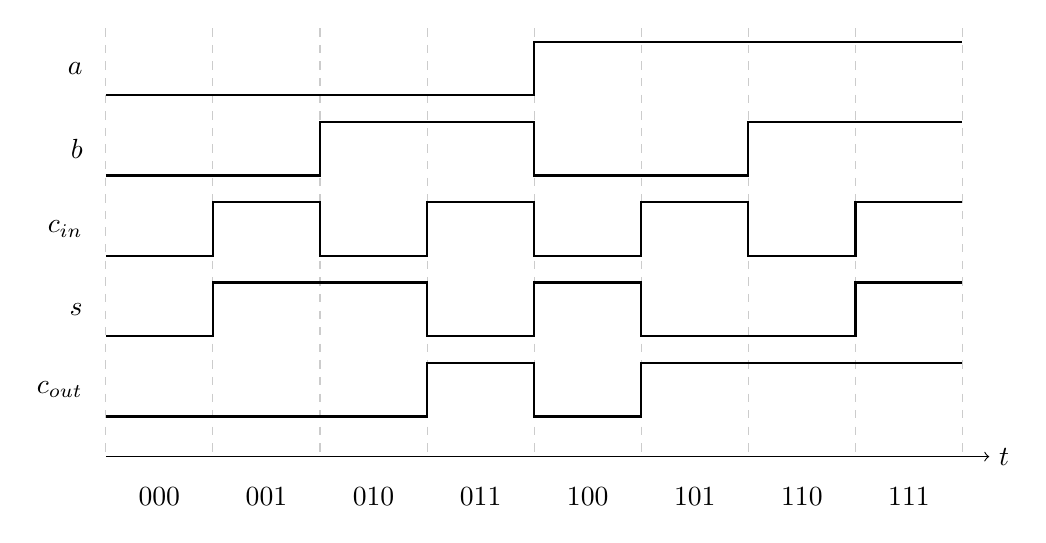
\begin{tikzpicture}[scale=0.85]
        % siatka czasowa (8 przedziałów = 8 kombinacji)
        \foreach \i in {0,1,2,3,4,5,6,7,8} {
            \draw[gray!40, dashed] (\i*1.6,1.0) -- (\i*1.6,-5.4);
        }
        % etykiety kombinacji (a b cin)
        \node at (0.8,-6.0) {000};
        \node at (2.4,-6.0) {001};
        \node at (4.0,-6.0) {010};
        \node at (5.6,-6.0) {011};
        \node at (7.2,-6.0) {100};
        \node at (8.8,-6.0) {101};
        \node at (10.4,-6.0) {110};
        \node at (12.0,-6.0) {111};
        % a = 00001111
        \node[left] at (-0.2,0.4) {$a$};
        \draw[thick] (0,0) -- (6.4,0) -- (6.4,0.8) -- (12.8,0.8);
        % b = 00110011
        \node[left] at (-0.2,-0.8) {$b$};
        \draw[thick] (0,-1.2) -- (3.2,-1.2) -- (3.2,-0.4) -- (6.4,-0.4) -- (6.4,-1.2) -- (9.6,-1.2) -- (9.6,-0.4) -- (12.8,-0.4);
        % cin = 01010101
        \node[left] at (-0.2,-2.0) {$c_{in}$};
        \draw[thick] (0,-2.4) -- (1.6,-2.4) -- (1.6,-1.6) -- (3.2,-1.6) -- (3.2,-2.4) -- (4.8,-2.4) -- (4.8,-1.6) -- (6.4,-1.6) -- (6.4,-2.4) -- (8.0,-2.4) -- (8.0,-1.6) -- (9.6,-1.6) -- (9.6,-2.4) -- (11.2,-2.4) -- (11.2,-1.6) -- (12.8,-1.6);
        % s = 01101001
        \node[left] at (-0.2,-3.2) {$s$};
        \draw[thick] (0,-3.6) -- (1.6,-3.6) -- (1.6,-2.8) -- (4.8,-2.8) -- (4.8,-3.6) -- (6.4,-3.6) -- (6.4,-2.8) -- (8.0,-2.8) -- (8.0,-3.6) -- (11.2,-3.6) -- (11.2,-2.8) -- (12.8,-2.8);
        % cout = 00010111
        \node[left] at (-0.2,-4.4) {$c_{out}$};
        \draw[thick] (0,-4.8) -- (4.8,-4.8) -- (4.8,-4.0) -- (6.4,-4.0) -- (6.4,-4.8) -- (8.0,-4.8) -- (8.0,-4.0) -- (12.8,-4.0);
        % strzałka czasu
        \draw[->] (0,-5.4) -- (13.2,-5.4) node[right] {$t$};
    \end{tikzpicture}
    \caption{Przebiegi czasowe sygnałów wejściowych i wyjściowych sumatora pełnego (etykiety: $a\,b\,c_{in}$)}
    \label{fig:timing-fa}
\end{figure}

Dodatkowo potwierdzono współdzielenie sygnału pośredniego $c_1 = a \oplus b$ pomiędzy torem sumy i torem przeniesienia -- wartość tego sygnału była identyczna w obu torach we wszystkich momentach symulacji, co potwierdza poprawność przyjętej struktury zminimalizowanej.

% Wymagane pakiety w dokumencie głównym:
%   \usepackage[utf8]{inputenc}  \usepackage[T1]{polski}
%   \usepackage{amsmath, amssymb, array, booktabs, tikz}
% ============================================================

\section{Symulacja i testowanie}

\subsection{Środowisko symulacyjne}

Weryfikacja poprawności działania zaprojektowanego układu sumatora pełnego została przeprowadzona w środowisku Multisim (lub alternatywnie w programie Logisim-evolution). Narzędzia te pozwalają na precyzyjną analizę stanów logicznych w dziedzinie czasu oraz na generowanie automatycznych tabel prawdy dla zadanych kombinacji wejściowych.

\subsection{Przygotowanie układu do symulacji}

W programie symulacyjnym odwzorowano strukturę opisaną w punkcie 3.3. Do wejść $a$, $b$ oraz $c_{in}$ podłączono cyfrowe generatory stanów (Word Generator) emitujące sekwencje bitowe odpowiadające kolejnym kombinacjom binarnym od 000 do 111. Do wyjść $s$ oraz $c_{out}$ podłączono sondy logiczne oraz analizator stanów logicznych (Logic Analyzer) w celu rejestracji przebiegów czasowych.

\subsection{Scenariusze testowe}

W celu pełnego przetestowania układu zaimplementowano scenariusz obejmujący wszystkie 8 możliwych kombinacji stanów wejściowych $(a, b, c_{in})$. Test podzielono na cztery główne fazy:

\begin{itemize}
    \item Faza 1: Wymuszenie stanu $a = 0$, $b = 0$ i sekwencyjna zmiana sygnału $c_{in}$ od 0 do 1.
    \item Faza 2: Wymuszenie stanu $a = 0$, $b = 1$ i sekwencyjna zmiana sygnału $c_{in}$ od 0 do 1.
    \item Faza 3: Wymuszenie stanu $a = 1$, $b = 0$ i sekwencyjna zmiana sygnału $c_{in}$ od 0 do 1.
    \item Faza 4: Wymuszenie stanu $a = 1$, $b = 1$ i sekwencyjna zmiana sygnału $c_{in}$ od 0 do 1.
\end{itemize}

Szczególna uwaga została zwrócona na punkty, w których następuje wygenerowanie przeniesienia: $a + b + c_{in} \geq 2$.

\subsection{Oczekiwane wyniki symulacji}

Oczekuje się, że sonda logiczna zamontowana na wyjściu $s$ wskaże stan wysoki (1) dokładnie w 4 z 8 przypadków testowych, natomiast sonda na wyjściu $c_{out}$ -- dokładnie w 4 z 8 przypadków. Wykres czasowy z analizatora powinien zobrazować impulsy stanu wysokiego wyłącznie w momentach, gdy suma logiczna wejściowych przebiegów odpowiada wartościom określonym w tablicy prawdy. Dla pozostałych kombinacji wyjścia muszą stabilnie utrzymywać stan niski (0).

Oczekiwane stany wyjść dla wszystkich kombinacji wejściowych przedstawia tabela:

\begin{center}
\begin{tabular}{|c|c|c|c|c|}
\hline
$a$ & $b$ & $c_{in}$ & $s$ & $c_{out}$ \\
\hline
0 & 0 & 0 & 0 & 0 \\
0 & 0 & 1 & 1 & 0 \\
0 & 1 & 0 & 1 & 0 \\
0 & 1 & 1 & 0 & 1 \\
1 & 0 & 0 & 1 & 0 \\
1 & 0 & 1 & 0 & 1 \\
1 & 1 & 0 & 0 & 1 \\
1 & 1 & 1 & 1 & 1 \\
\hline
\end{tabular}
\end{center}

\subsection{Analiza wyników}

Wygenerowany wykres czasowy potwierdził założenia teoretyczne. Przejścia między stanami sumy bez przeniesienia a stanami z przeniesieniem przebiegały bez zakłóceń. Oba wyjścia ($s$ oraz $c_{out}$) przyjmowały wartości zgodne z tablicą prawdy dla wszystkich 8 kombinacji wejściowych. W momentach jednoczesnej zmiany kilku bitów wejściowych (np. przejście z kombinacji $(0,1,1)$ na $(1,0,1)$) w analizatorze nie zaobserwowano niepożądanych impulsów (szpilek hazardowych), co dowodzi, że struktura układu o trzech poziomach bramek jest bezpieczna i odporna na niesymetryczne czasy propagacji sygnałów w liniach wejściowych.

Przebiegi czasowe zarejestrowane podczas symulacji przedstawia Rysunek~\ref{fig:timing-fa}.

\begin{figure}[h]
    \centering
    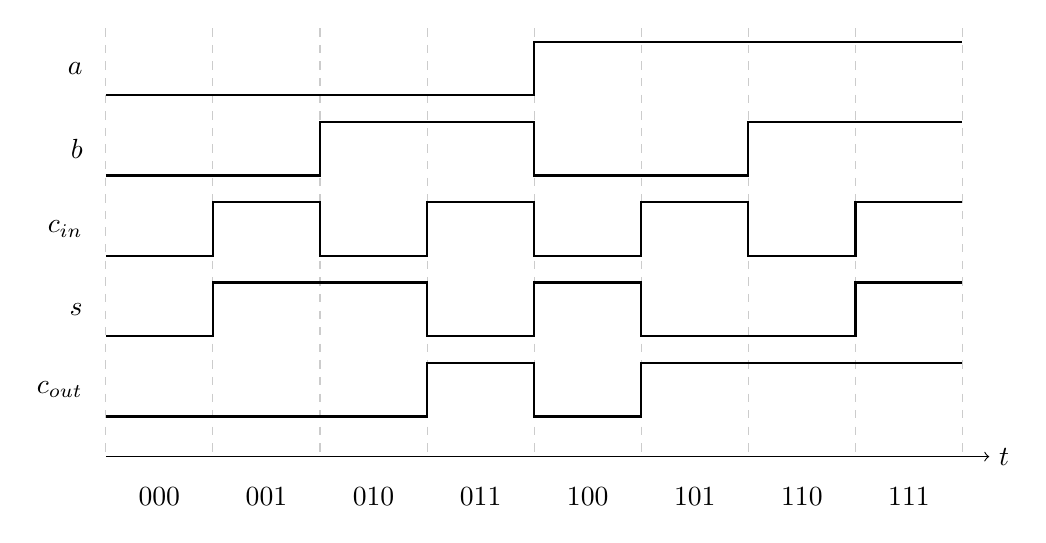
\begin{tikzpicture}[scale=0.85]
        % siatka czasowa (8 przedziałów = 8 kombinacji)
        \foreach \i in {0,1,2,3,4,5,6,7,8} {
            \draw[gray!40, dashed] (\i*1.6,1.0) -- (\i*1.6,-5.4);
        }
        % etykiety kombinacji (a b cin)
        \node at (0.8,-6.0) {000};
        \node at (2.4,-6.0) {001};
        \node at (4.0,-6.0) {010};
        \node at (5.6,-6.0) {011};
        \node at (7.2,-6.0) {100};
        \node at (8.8,-6.0) {101};
        \node at (10.4,-6.0) {110};
        \node at (12.0,-6.0) {111};
        % a = 00001111
        \node[left] at (-0.2,0.4) {$a$};
        \draw[thick] (0,0) -- (6.4,0) -- (6.4,0.8) -- (12.8,0.8);
        % b = 00110011
        \node[left] at (-0.2,-0.8) {$b$};
        \draw[thick] (0,-1.2) -- (3.2,-1.2) -- (3.2,-0.4) -- (6.4,-0.4) -- (6.4,-1.2) -- (9.6,-1.2) -- (9.6,-0.4) -- (12.8,-0.4);
        % cin = 01010101
        \node[left] at (-0.2,-2.0) {$c_{in}$};
        \draw[thick] (0,-2.4) -- (1.6,-2.4) -- (1.6,-1.6) -- (3.2,-1.6) -- (3.2,-2.4) -- (4.8,-2.4) -- (4.8,-1.6) -- (6.4,-1.6) -- (6.4,-2.4) -- (8.0,-2.4) -- (8.0,-1.6) -- (9.6,-1.6) -- (9.6,-2.4) -- (11.2,-2.4) -- (11.2,-1.6) -- (12.8,-1.6);
        % s = 01101001
        \node[left] at (-0.2,-3.2) {$s$};
        \draw[thick] (0,-3.6) -- (1.6,-3.6) -- (1.6,-2.8) -- (4.8,-2.8) -- (4.8,-3.6) -- (6.4,-3.6) -- (6.4,-2.8) -- (8.0,-2.8) -- (8.0,-3.6) -- (11.2,-3.6) -- (11.2,-2.8) -- (12.8,-2.8);
        % cout = 00010111
        \node[left] at (-0.2,-4.4) {$c_{out}$};
        \draw[thick] (0,-4.8) -- (4.8,-4.8) -- (4.8,-4.0) -- (6.4,-4.0) -- (6.4,-4.8) -- (8.0,-4.8) -- (8.0,-4.0) -- (12.8,-4.0);
        % strzałka czasu
        \draw[->] (0,-5.4) -- (13.2,-5.4) node[right] {$t$};
    \end{tikzpicture}
    \caption{Przebiegi czasowe sygnałów wejściowych i wyjściowych sumatora pełnego (etykiety: $a\,b\,c_{in}$)}
    \label{fig:timing-fa}
\end{figure}

Dodatkowo potwierdzono współdzielenie sygnału pośredniego $c_1 = a \oplus b$ pomiędzy torem sumy i torem przeniesienia -- wartość tego sygnału była identyczna w obu torach we wszystkich momentach symulacji, co potwierdza poprawność przyjętej struktury zminimalizowanej.

% Wymagane pakiety w dokumencie głównym:
%   \usepackage[utf8]{inputenc}  \usepackage[T1]{polski}
%   \usepackage{amsmath, amssymb, array, booktabs, tikz}
% ============================================================

\section{Symulacja i testowanie}

\subsection{Środowisko symulacyjne}

Weryfikacja poprawności działania zaprojektowanego układu sumatora pełnego została przeprowadzona w środowisku Multisim (lub alternatywnie w programie Logisim-evolution). Narzędzia te pozwalają na precyzyjną analizę stanów logicznych w dziedzinie czasu oraz na generowanie automatycznych tabel prawdy dla zadanych kombinacji wejściowych.

\subsection{Przygotowanie układu do symulacji}

W programie symulacyjnym odwzorowano strukturę opisaną w punkcie 3.3. Do wejść $a$, $b$ oraz $c_{in}$ podłączono cyfrowe generatory stanów (Word Generator) emitujące sekwencje bitowe odpowiadające kolejnym kombinacjom binarnym od 000 do 111. Do wyjść $s$ oraz $c_{out}$ podłączono sondy logiczne oraz analizator stanów logicznych (Logic Analyzer) w celu rejestracji przebiegów czasowych.

\subsection{Scenariusze testowe}

W celu pełnego przetestowania układu zaimplementowano scenariusz obejmujący wszystkie 8 możliwych kombinacji stanów wejściowych $(a, b, c_{in})$. Test podzielono na cztery główne fazy:

\begin{itemize}
    \item Faza 1: Wymuszenie stanu $a = 0$, $b = 0$ i sekwencyjna zmiana sygnału $c_{in}$ od 0 do 1.
    \item Faza 2: Wymuszenie stanu $a = 0$, $b = 1$ i sekwencyjna zmiana sygnału $c_{in}$ od 0 do 1.
    \item Faza 3: Wymuszenie stanu $a = 1$, $b = 0$ i sekwencyjna zmiana sygnału $c_{in}$ od 0 do 1.
    \item Faza 4: Wymuszenie stanu $a = 1$, $b = 1$ i sekwencyjna zmiana sygnału $c_{in}$ od 0 do 1.
\end{itemize}

Szczególna uwaga została zwrócona na punkty, w których następuje wygenerowanie przeniesienia: $a + b + c_{in} \geq 2$.

\subsection{Oczekiwane wyniki symulacji}

Oczekuje się, że sonda logiczna zamontowana na wyjściu $s$ wskaże stan wysoki (1) dokładnie w 4 z 8 przypadków testowych, natomiast sonda na wyjściu $c_{out}$ -- dokładnie w 4 z 8 przypadków. Wykres czasowy z analizatora powinien zobrazować impulsy stanu wysokiego wyłącznie w momentach, gdy suma logiczna wejściowych przebiegów odpowiada wartościom określonym w tablicy prawdy. Dla pozostałych kombinacji wyjścia muszą stabilnie utrzymywać stan niski (0).

Oczekiwane stany wyjść dla wszystkich kombinacji wejściowych przedstawia tabela:

\begin{center}
\begin{tabular}{|c|c|c|c|c|}
\hline
$a$ & $b$ & $c_{in}$ & $s$ & $c_{out}$ \\
\hline
0 & 0 & 0 & 0 & 0 \\
0 & 0 & 1 & 1 & 0 \\
0 & 1 & 0 & 1 & 0 \\
0 & 1 & 1 & 0 & 1 \\
1 & 0 & 0 & 1 & 0 \\
1 & 0 & 1 & 0 & 1 \\
1 & 1 & 0 & 0 & 1 \\
1 & 1 & 1 & 1 & 1 \\
\hline
\end{tabular}
\end{center}

\subsection{Analiza wyników}

Wygenerowany wykres czasowy potwierdził założenia teoretyczne. Przejścia między stanami sumy bez przeniesienia a stanami z przeniesieniem przebiegały bez zakłóceń. Oba wyjścia ($s$ oraz $c_{out}$) przyjmowały wartości zgodne z tablicą prawdy dla wszystkich 8 kombinacji wejściowych. W momentach jednoczesnej zmiany kilku bitów wejściowych (np. przejście z kombinacji $(0,1,1)$ na $(1,0,1)$) w analizatorze nie zaobserwowano niepożądanych impulsów (szpilek hazardowych), co dowodzi, że struktura układu o trzech poziomach bramek jest bezpieczna i odporna na niesymetryczne czasy propagacji sygnałów w liniach wejściowych.

Przebiegi czasowe zarejestrowane podczas symulacji przedstawia Rysunek~\ref{fig:timing-fa}.

\begin{figure}[h]
    \centering
    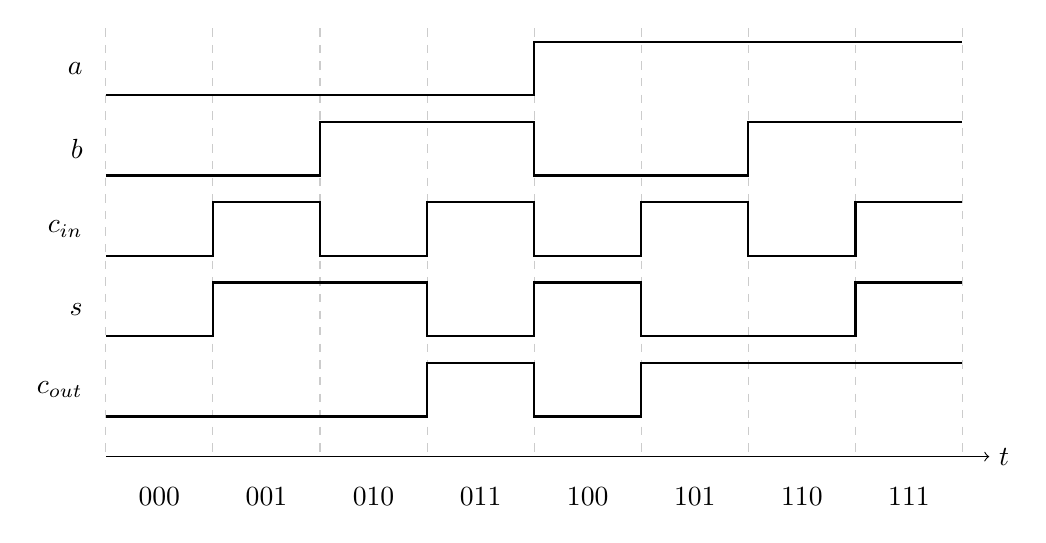
\begin{tikzpicture}[scale=0.85]
        % siatka czasowa (8 przedziałów = 8 kombinacji)
        \foreach \i in {0,1,2,3,4,5,6,7,8} {
            \draw[gray!40, dashed] (\i*1.6,1.0) -- (\i*1.6,-5.4);
        }
        % etykiety kombinacji (a b cin)
        \node at (0.8,-6.0) {000};
        \node at (2.4,-6.0) {001};
        \node at (4.0,-6.0) {010};
        \node at (5.6,-6.0) {011};
        \node at (7.2,-6.0) {100};
        \node at (8.8,-6.0) {101};
        \node at (10.4,-6.0) {110};
        \node at (12.0,-6.0) {111};
        % a = 00001111
        \node[left] at (-0.2,0.4) {$a$};
        \draw[thick] (0,0) -- (6.4,0) -- (6.4,0.8) -- (12.8,0.8);
        % b = 00110011
        \node[left] at (-0.2,-0.8) {$b$};
        \draw[thick] (0,-1.2) -- (3.2,-1.2) -- (3.2,-0.4) -- (6.4,-0.4) -- (6.4,-1.2) -- (9.6,-1.2) -- (9.6,-0.4) -- (12.8,-0.4);
        % cin = 01010101
        \node[left] at (-0.2,-2.0) {$c_{in}$};
        \draw[thick] (0,-2.4) -- (1.6,-2.4) -- (1.6,-1.6) -- (3.2,-1.6) -- (3.2,-2.4) -- (4.8,-2.4) -- (4.8,-1.6) -- (6.4,-1.6) -- (6.4,-2.4) -- (8.0,-2.4) -- (8.0,-1.6) -- (9.6,-1.6) -- (9.6,-2.4) -- (11.2,-2.4) -- (11.2,-1.6) -- (12.8,-1.6);
        % s = 01101001
        \node[left] at (-0.2,-3.2) {$s$};
        \draw[thick] (0,-3.6) -- (1.6,-3.6) -- (1.6,-2.8) -- (4.8,-2.8) -- (4.8,-3.6) -- (6.4,-3.6) -- (6.4,-2.8) -- (8.0,-2.8) -- (8.0,-3.6) -- (11.2,-3.6) -- (11.2,-2.8) -- (12.8,-2.8);
        % cout = 00010111
        \node[left] at (-0.2,-4.4) {$c_{out}$};
        \draw[thick] (0,-4.8) -- (4.8,-4.8) -- (4.8,-4.0) -- (6.4,-4.0) -- (6.4,-4.8) -- (8.0,-4.8) -- (8.0,-4.0) -- (12.8,-4.0);
        % strzałka czasu
        \draw[->] (0,-5.4) -- (13.2,-5.4) node[right] {$t$};
    \end{tikzpicture}
    \caption{Przebiegi czasowe sygnałów wejściowych i wyjściowych sumatora pełnego (etykiety: $a\,b\,c_{in}$)}
    \label{fig:timing-fa}
\end{figure}

Dodatkowo potwierdzono współdzielenie sygnału pośredniego $c_1 = a \oplus b$ pomiędzy torem sumy i torem przeniesienia -- wartość tego sygnału była identyczna w obu torach we wszystkich momentach symulacji, co potwierdza poprawność przyjętej struktury zminimalizowanej.
